\chapter{Bandas de energía en el grafeno}\label{cap.2}
\markboth{Bandas de energía en el grafeno}{Bandas de energía en el grafeno}
En este capítulo se estudiará la estructura cristalina del grafeno, la cual al no ser una red de Bravais tiene propiedades de simetría distintas que surgen debido a que su celda de Wigner-Seitz tiene dos elementos. Estas características modifican el enfoque que se usa, por ejemplo al hallar la función de onda de Bloch del sistema, esta debe estar expresada como una combinación lineal de las dos sub-redes formadas por cada elemento de la celda de Wigner-Seitz, a diferencia del caso de una red de Bravais cuyas celdas de Wigner-Seitz constan de un elemento, por lo que su función de onda de Bloch no depende de dos sub-redes.\\ 
Para describir la dinámica de los electrones en el grafeno se usa el modelo del Tight-Binding. Sin embargo para hacer esto es necesario definir los electrones cuyos comportamientos serán descritos. Estos serán los electrones que ocupan los orbitales $p_z$ de los átomos de carbono, y solo se considerarán las interacciones entre estos y los iones positivos de la red cristalina, cuyos elementos son los núcleos y los demás electrones del átomo de carbono.\\
A partir de esto se observará que existen dos bandas de energía, las cuales se intersectan en los llamados \emph{puntos de Dirac}. Estos son iguales a los puntos de la red recíproca del grafeno, por lo que se tienen dos clases de puntos de Dirac, los cuales tienen Hamiltonianos distintos como se verá en el siguiente capítulo. 
% En este capítulo se estudiará la estructura cristalina del grafeno y sus elementos, así como los tipos de simetría que esta tiene. Se sigue la notación mostrada en \cite{Lomer1955} para las representar las matrices.



\section{Estructura cristalina} \renewcommand{\thefootnote}{\arabic{footnote}} % numeración por símbolos
\lhead[\thepage]{\thesection. Estructura cristalina}
\subsection{Elementos de la estructura cristalina}
% TODO: ¿Cuál es la estructura cristalina del grafeno?
% ¿Cuál es la evidencia de tal estructura cristalina?
% ¿Cuál es la celda unitaria del grafeno?
% ¿Cuál es la celda de Wigner-Seitz del grafeno?
El grafeno es un material bidimensional formado por átomos de carbono que se encuentran unidos mediantes enlaces tipo $\sigma$, formando así un arreglo hexagonal como se muestra en la Figura \ref{fig:wigner}.

\begin{figure}[!httb]
	\centering
	\includesvg[width=0.4\textwidth]{figures/wigner.svg}
	\caption{Estructura cristalina y las celdas de Wigner-Seitz del grafeno}
	\label{fig:wigner}
\end{figure}

\noindent La celda unitaria de una estructura cristalina es definida como una porción de la red, la cual genera la estructura cristalina. Esta definición permite definir diferentes tipos de celda unitarias para el grafeno, siendo la más evidente la celda en forma de hexágono con átomos de carbono en sus vértices. Sin embargo, existe otro tipo de celda unitaria, llamada \emph{celda de Wigner-Seitz}, la cual será la utilizada para estudiar la estructura cristalina del grafeno. Esta es la celda que rodea a un punto de la estructura cristalina tal que los vectores que van desde este hacia los puntos más cercanos intersectan de forma perpendicular a los lados de la celda, dividiendo a la mitad a estos vectores. Para el caso del grafeno esta tiene la forma de un paralelogramo, aunque existen tres orientaciones distintas para estas (ver Fig. \ref{fig:wigner}), con dos puntos de la red contenidos en este. Esto permite clasificar los puntos de la red cristalina en dos clases, las cuales forman dos redes triangulares.

\begin{figure}[!httb]
	\centering
	\includesvg[width=0.4\textwidth]{figures/cristalline.svg}
	\caption{Vectores primitivos de la estructura cristalina del grafeno}
	\label{fig:crystalline}
\end{figure}

Dado que los vectores primitivos son definidos como los vectores que conectan dos puntos consecutivos de una estructura cristalina, los vectores primitivos asociados a cada sub-red triangular serán $\vec{a}_1$ y $\vec{a}_2$ (ver Fig. \ref{fig:crystalline}). Estos se pueden representar en la base $\left\{\hat{x},\hat{y}\right\}$ como
\begin{equation}
	\vec{a}_1 = \frac{a\sqrt{3}}{2}\left(\hat{x}+\sqrt{3} \hat{y}\right),\hspace{0.5cm}\vec{a}_2= \frac{a \sqrt{3}}{2}\left(-\hat{x}+\sqrt{3} \hat{y}\right)\label{eq:primitive}
\end{equation}
Al desplazar la celda de Wigner-Seitz en un vector que es igual a una combinación lineal de coeficientes enteros de los vectores primitivos se puede generar la estructura cristalina del grafeno. Por lo que estos vectores serán de utilidad cuando se estudien las propiedades de simetría de la estructura cristalina.\par
La red cristalina está expresada en el espacio de posiciones, esto no es conveniente cuando se requiere una expresión que no dependa de estas. Al realizar el cambio a el espacio de vectores de onda $\vec{k}$, la red cristalina asociada a este tiene como vectores primitivos a $\vec{a}_1^{\ast}$ y $\vec{a}_2^{\ast}$, los cuales satisfacen la relación 
\begin{equation}
	\vec{a}^{\ast}_i\cdot \vec{a}_j = 2\pi\delta_{ij} \quad \left(i,j = 1,2\right).
\end{equation}
para poder mantener la periodicidad de la red cristalina. Esta red cristalina es llamada \emph{red recíproca}.\\ Los vectores primitivos de la red recíproca se pueden expresar en la base $\left\{\hat{x}, \hat{y}\right\}$ como
% A partir de los vectores primitivos se pueden obtener los vectores $\vec{a}_1^{\ast}$, $\vec{a}_2^{\ast}$, definidos como los vectores que cumplen la relación \cite{Bradley2009}:
% \begin{equation}
% 	\vec{a}^{\ast}_i\cdot \vec{a}_j = 2\pi\delta_{ij} \quad \left(i,j = 1,2\right).
% \end{equation}
% Estos vectores pueden formar una estructura cristalina, llamada \emph{red recíproca}, por lo que son vectores primitivos de esta última. En la base $\left\{\hat{x}, \hat{y}\right\}$ se expresan como 
\begin{equation}
	\vec{a}^{\ast}_1 = \frac{2\pi}{3a}\left(\sqrt{3}\hat{x}+\hat{y}\right),\hspace{0.5cm}\vec{a}^{\ast}_2= \frac{2\pi}{3a}\left(-\sqrt{3}\hat{x}+\hat{y}\right).\label{eq:recipprimitive}
\end{equation}
A continuación se muestran los puntos de la red recíproca más cercanos al origen de coordenadas
\begin{equation}
  \begin{aligned}[b]
    \vec{k} = \hspace{0.3cm}\frac{4\pi}{3\sqrt{3}a}\hat{x}\hspace{1.5cm} \vec{k} = \hspace{0.3cm}\frac{2\pi}{3\sqrt{3}a} \hat{x}+ \frac{2\pi}{3a} \hat{y} \hspace{1.5cm} \vec{k} = \hspace{0.3cm}\frac{2\pi}{3\sqrt{3}a} \hat{x} -\frac{2\pi}{3a} \hat{y}                                                                          \\
	\vec{k} = -\frac{4\pi}{3\sqrt{3}a}\hat{x}  \hspace{1.5cm} \vec{k} = -\frac{2\pi}{3\sqrt{3}a} \hat{x}+\frac{2\pi}{3a} \hat{y} \hspace{1.5cm} \vec{k} = -\frac{2\pi}{3\sqrt{3}a} \hat{x}-\frac{2\pi}{3a} \hat{y}
\end{aligned}
\end{equation}
Para el caso de la red recíproca, la celda de Wigner-Seitz es llamada \emph{zona de Brillouin}. Esta tiene la forma de un paralelogramo que contiene dos puntos de la red recíproca, ya que la red recíproca tiene un arreglo hexagonal, al igual que la estructura cristalina. Por ende, la red recíproca se pueden dividir en dos sub-redes triangulares y tiene las mismas propiedades de simetría que la estructura cristalina inicial.
\subsection{Propiedades de simetría}
El grafeno tiene ciertas transformaciones de simetría que se definen como aquellas que dejan invariante a la estructura cristalina. 
\begin{figure}[!httb]
    \centering
    \begin{subfigure}[b]{0.3\linewidth}
        \centering
        \includesvg[width=\textwidth]{figures/twofold1.svg}
        \caption{Simetrías de reflexión\\\hfill}
        \label{fig:twofold}
    \end{subfigure}
    \hfill
    \begin{subfigure}[b]{0.3\linewidth}
        \centering
        \includesvg[width=\textwidth]{figures/rotation.svg}
        \caption{Simetrías de rotación alrededor del eje z}
        \label{fig:rotation}
    \end{subfigure}
    \hfill
    \begin{subfigure}[b]{0.3\linewidth}
        \centering
        \includesvg[width=\textwidth]{figures/inversion.svg}
        \caption{Inversión alrededor del origen de coordenadas}
        \label{fig:inversion}
    \end{subfigure}
    \caption{Simetrías de reflexión, rotación e inversión del grafeno}
\end{figure}

Las reflexiones de la Figura \ref{fig:twofold} se pueden representar en la base $\left\{\hat{x},\hat{y}\right\}$ como 
\begin{align}
  \begin{split}
    s_1 = \begin{pmatrix}
  1 & 0\\
  0 & -1
  \end{pmatrix}\hspace{1.4cm}s_2 = \begin{pmatrix}
      \frac{1}{2} & \frac{\sqrt{3}}{2}\\
      \frac{\sqrt{3}}{2} & -\frac{1}{2}
      \end{pmatrix} \hspace{1.3cm} s_3 = \begin{pmatrix}
      -\frac{1}{2} & \frac{\sqrt{3}}{2} \\
\frac{\sqrt{3}}{2} & \frac{1}{2}
    \end{pmatrix}\\
     s_4 = \begin{pmatrix}
    -1 & 0\\
    0 & 1
  \end{pmatrix}\hspace{0.7cm} s_5 = \begin{pmatrix}
    -\frac{1}{2} & -\frac{\sqrt{3}}{2} \\
    -\frac{\sqrt{3}}{2} & \frac{1}{2}
  \end{pmatrix} \hspace{0.7cm} s_6 = \begin{pmatrix}
  \frac{1}{2} & -\frac{\sqrt{3}}{2} \\
  -\frac{\sqrt{3}}{2} & -\frac{1}{2}
  \end{pmatrix}
   \end{split}
\end{align}
Y las rotaciones de la Figura \ref{fig:rotation} se puede representar como
\begin{align}
  \begin{split}
    e = \begin{pmatrix}
       1 & 0\\
       0 & 1 
      \end{pmatrix} \hspace{0.9cm} r^1 = \begin{pmatrix}
    \frac{1}{2} & -\frac{\sqrt{3}}{2}\\
    \frac{\sqrt{3}}{2} & \frac{1}{2}
  \end{pmatrix} \hspace{0.9cm} r^2 = \begin{pmatrix}
  -\frac{1}{2} & -\frac{\sqrt{3}}{2} \\
  \frac{\sqrt{3}}{2} & -\frac{1}{2}
  \end{pmatrix}\\
    r^3 = \begin{pmatrix}
      -1 & 0\\
 0 & -1
    \end{pmatrix} \hspace{0.7cm} r^4 = \begin{pmatrix}
    -\frac{1}{2} & \frac{\sqrt{3}}{2} \\
    -\frac{\sqrt{3}}{2} & -\frac{1}{2}
    \end{pmatrix} \hspace{0.7cm} r^5 = \begin{pmatrix}
  \frac{1}{2} & \frac{\sqrt{3}}{2}\\
  -\frac{\sqrt{3}}{2} & \frac{1}{2}
  \end{pmatrix} 
   \end{split}
\end{align}
Por último la simetría de inversión (ver Fig. \ref{fig:inversion}) es representada por
\begin{equation}
   I = \begin{pmatrix}
     -1 & 0\\
     0 & -1
   \end{pmatrix}.
\end{equation}
Se puede notar que la matriz que representa a la simetría de inversión es la misma que la que representación a la rotación $r^3$. Por lo que al realizar el análisis de las simetrías del grafeno la simetría de inversión no se mencionará como tal, sino como una de las simetrías de rotación.\par
Además de las simetrías anteriores que dejan un punto invariante, como el eje de coordenadas, existen otras que no fijan un punto en particular. Por ende, estas no pueden representadas por un transformación lineal, sino por una transformación afín. Unas de estas son las simetrías de traslación, las cuales para el caso de una estructura cristalina hexagonal son
\begin{equation}
  T = \left\{\vec{w} \mid \vec{w} = \alpha \vec{a}_1 + \beta \vec{a}_2\text{, donde }\alpha,\beta \in \mathbb{Z}\right\}
\end{equation}
% %WARNING: Old content of the symmetries
% Se definen los grupos espacios como los grupos de simetrías que dejan invariantes al patrón de un cristal. Siguiendo esto una traslación en $\vec{a}_1$ deja invariante a la estructura cristalina, y por ende corresponde a un elemento de este grupo. De la Figura \ref{fig:crystalline} se obtiene que las traslaciones correspondientes a los vectores $\alpha\vec{a}_1+\beta\vec{a}_2$, donde $\alpha$ y $\beta$ son números enteros, dejan invariante a la estrutura cristalina del grafeno. Esto es equivalente a que es invariante a traslaciones de algún vector primitivo de algún par de vectores de primitivos.\\ Además se observa que las rotaciones de $\frac{2\pi}{3}$ y $\frac{4\pi}{3}$ alrededor del origen también corresponden a elementos del grupo espacio, estos se representan en la base $\{\hat{x},\hat{y}\}$ como
% \begin{equation}
% 	R = \begin{pmatrix}
% 		-\frac{1}{2}       & -\frac{\sqrt{3}}{2} \\
% 		\frac{\sqrt{3}}{2} & -\frac{1}{2}
% 	\end{pmatrix}\Bigg| \begin{matrix}
% 		0 \\ 0
% 	\end{matrix},\quad R ^{-1} = \begin{pmatrix}
% 		-\frac{1}{2}        & \frac{\sqrt{3}}{2} \\
% 		-\frac{\sqrt{3}}{2} & -\frac{1}{2}       \\
% 	\end{pmatrix}\Bigg| \begin{matrix}
% 		0 \\0
% 	\end{matrix}\quad y \quad E = \begin{pmatrix}
% 		1 & 0 \\
% 		0 & 1
% 	\end{pmatrix}\Bigg| \begin{matrix}
% 		0 \\ 0
% 	\end{matrix}.
% \end{equation}
% Definiendo los planos $(z,x_1)$, $(z,x_2)$, $(z,x_3)$ como en la Figura \ref{fig:symmetry} se tienen simetrías de espejo.
%
% \begin{figure}[!httb]
% 	\centering
% 	\includesvg[width=0.4\textwidth]{figures/symmetry.svg}
% 	\caption{Planos de simetría y rotación}
% 	\label{fig:symmetry}
% \end{figure}
%
% \noindent Estas se representan en la base $\left\{\hat{x},\hat{y}\right\}$ como
% \begin{equation}
% 	X_1 = \begin{pmatrix}
% 		1 & 0  \\
% 		0 & -1
% 	\end{pmatrix}\Bigg| \begin{matrix}
% 		0 \\ -a
% 	\end{matrix},\quad X_2 = \begin{pmatrix}
% 		-\frac{1}{2}       & \frac{\sqrt{3}}{2} \\
% 		\frac{\sqrt{3}}{2} & \frac{1}{2}
% 	\end{pmatrix}\Bigg| \begin{matrix}
% 		-\frac{a\sqrt{3}}{2} \\
% 		\frac{a}{2}
% 	\end{matrix}, \quad X_3 = \begin{pmatrix}
% 		- \frac{1}{2}       & - \frac{\sqrt{3}}{2} \\
% 		-\frac{\sqrt{3}}{2} & \frac{1}{2}
% 	\end{pmatrix}\Bigg| \begin{matrix}
% 		\frac{a \sqrt{3}}{2} \\
% 		\frac{a}{2}
% 	\end{matrix}
% \end{equation}
% Nótese que estas operaciones intercambian una clase de puntos con la otra. En cambio, las simetrías espejo respecto de los planos $\left(z,y_1\right)$, $\left(z,y_2\right)$, $\left(z,y_3\right)$ no intercambian estas. Sin embargo esto no cambia la forma de la estructura cristalina pues lo importante es que esta sea formada por las celda de Wigner-Seitz independientemente del orden de los puntos elegidos, ya que en la celda unitaria se encuentran dos elementos de clases distintas.\\
% La representación matricial de las últimas es
% \begin{equation}
% 	Y_1 = \begin{pmatrix}
% 		\frac{1}{2}         & -\frac{\sqrt{3}}{2} \\
% 		-\frac{\sqrt{3}}{2} & -\frac{1}{2}
% 	\end{pmatrix}\Bigg| \begin{matrix}
% 		0 \\ 0
% 	\end{matrix}, \quad Y_2 =\begin{pmatrix}
% 		-1 & 0 \\
% 		0  & 1
% 	\end{pmatrix}\Bigg| \begin{matrix}
% 		0 \\ 0
% 	\end{matrix}\quad y \quad Y_3 = \begin{pmatrix}
% 		\frac{1}{2}        & \frac{\sqrt{3}}{2} \\
% 		\frac{\sqrt{3}}{2} & -\frac{1}{2}
% 	\end{pmatrix}\Bigg| \begin{matrix}
% 		0 \\ 0
% 	\end{matrix}
% \end{equation}
% Además se tiene la siguiente simetría cuya representación matricial es
% \begin{equation}
% 	W = \begin{pmatrix}
% 		\frac{1}{2}        & -\frac{\sqrt{3}}{2} \\
% 		\frac{\sqrt{3}}{2} & \frac{1}{2}
% 	\end{pmatrix}\Bigg| \begin{matrix}
% 		\frac{a \sqrt{3}}{2} \\
% 		\frac{a}{2}
% 	\end{matrix}
% \end{equation}
% La estructura cristalina del grafeno también tiene simetría de reflexión, por ejemplo, tomando como el punto de inversión a $I$ se tiene la representación de la transperación:
% \begin{equation}
% 	M = \begin{pmatrix}
% 		-1 & 0  \\
% 		0  & -1
% 	\end{pmatrix}\Bigg| \begin{matrix}
% 		\frac{a \sqrt{3}}{2} \\
% 		\frac{-3a}{2}
% 	\end{matrix}
% \end{equation}
% Se puede notar que todas las posibles transformaciones que dejan invariante al grafeno se generan de combinaciones de rotaciones, traslaciones, reflexiones, simetría espejo.\\
% Además se observa que estas transformaciones son en realidad mapeos afines, por lo que  siguiendo la notación de Seitz, se puede representar como $\left\{\mathcal{R}\mid \vec{t}\right\}$, donde $\mathcal{R}$ es una matriz de rotación y $\vec{t}$ representa una translación. Nótese que $t$ no es necesariamente una traslación que permite la conservación de la simetría del grafeno, como ejemplo se tiene que $X_1Y_2=\left\{M\mid -\frac{\vec{a}_1+\vec{a}_2}{3}\right\}$. Sin embargo, se encuentra que la parte matricial de estas transformaciones forma un grupo, cuyos elementos cumplen la relación mostrada en \cite{Lomer1955}.\\
% Se concluye que el grafeno tiene simetrías de traslación, rotación, reflexión y espejo. Además de ser invariante a mapeos afines generados por composiciones de estas.
\section{Grupo de simetría}
%TODO: Con lo anterior defina el grupo de simetría para estructura del grafeno
Los simetrías que mantienen un punto fijo satisfacen las relaciones
\begin{table}[!httb]
  \centering
  \begin{tabular}{|c | c c c c c c c c c c c c|}
    \hline
   & $e$ & $r^1$ & $r^2$ & $r^3$ & $r^4$ & $r^5$ & $s_1$ & $s_2$ & $s_3$ & $s_4$ & $s_5$ & $s_6$\\\hline
  $e$ & $e$ & $r^1$ & $r^2$ & $r^3$ & $r^4$ & $r^5$ & $s_1$ & $s_2$ & $s_3$ & $s_4$ & $s_5$ & $s_6$\\
  $r^1$ & $r^1$ & $r^2$ & $r^3$ & $r^4$ & $r^5$ & $e$ & $s_2$ & $s_3$ & $s_4$ & $s_5$ & $s_6$ & $s_1$\\
  $r^2$ & $r^2$ & $r^3$ & $r^4$ & $r^5$ & $e$ & $r^1$ & $s_3$ & $s_4$ & $s_5$ & $s_6$ & $s_1$ & $s_2$\\
  $r^3$ & $r^3$ & $r^4$ & $r^5$ & $e$ & $r^1$ & $r^2$ & $s_4$ & $s_5$ & $s_6$ & $s_1$ & $s_2$ & $s_3$\\
  $r^4$ & $r^4$ & $r^5$ & $e$ & $r^1$ & $r^2$ & $r^3$ & $s_5$ & $s_6$ & $s_1$ & $s_2$ & $s_3$ & $s_2$\\
  $r^5$ & $r^5$ & $e$ & $r^1$ & $r^2$ & $r^3$ & $r^4$ & $s_6$ & $s_5$ & $s_4$ & $s_3$ & $s_2$ & $s_1$\\
  $s_1$ & $s_1$ & $s_6$ & $s_5$ & $s_4$ & $s_3$ & $s_2$ & $e$ & $r^5$ & $r^4$ & $r^3$ & $r^2$ & $r^1$\\
  $s_2$ & $s_2$ & $s_1$ & $s_6$ & $s_5$ & $s_4$ & $s_3$ & $r^1$ & $e$ & $r^5$ & $r^4$ & $r^3$ & $r^2$\\
  $s_3$ & $s_3$ & $s_2$ & $s_1$ & $s_6$ & $s_5$ & $s_4$ & $r^2$ & $r^1$ & $e$ & $r^5$ & $r^4$ & $r^3$\\
  $s_4$ & $s_4$ & $s_3$ & $s_2$ & $s_1$ & $s_6$ & $s_5$ & $r^3$ & $r^2$ & $r^1$ & $e$ & $r^5$ & $r^4$\\
  $s_5$ & $s_5$ & $s_4$ & $s_3$ & $s_2$ & $s_1$ & $s_6$ & $r^4$ & $r^3$ & $r^2$ & $r^1$ & $e$ & $r^5$\\
  $s_6$ & $s_6$ & $s_5$ & $s_4$ & $s_3$ & $s_2$ & $s_1$ & $r^5$ & $r^4$ & $r^3$ & $r^2$ & $r^1$ & $e$\\\hline
  \end{tabular}
\end{table}

Por ende, estos forman un grupo. Este grupo es conocido como el \emph{grupo diédrico} del hexágono, y es denotado por $D_6$. Este es el grupo puntual de una estructura cristalina hexagonal. Es evidente que es un grupo finito, pero al hallar la suma directa con el grupo $T$ se genera el \emph{grupo espacial} de la estructura hexagonal. Este es un grupo infinito, ya que el grupo $T$ tiene infinitos elementos.
\section{Función de onda}
\subsection{Aspectos generales de la función de onda}
%TODO:
% Cuáles son las predicciones de una teoría cuántica sobre un sistema
% Cómo una función de onda define completamente un sistema cuántico
% Cómo se determina la función de onda 
% Cómo se determina el espectro de energías de un sistema cuántico
% Se puede expresar la función de onda de un sistema de muchas partículas en términos de una?
Antes de describir el comportamiento de los electrones en el grafeno es necesario mostrar el marco teórico que rige su dinámica. Empezando con una partícula, su estado es definido matemáticamente como un elemento de un espacio de Hilbert $\mathcal{H}$ ya la familia de estos genera ese espacio de Hilbert. Este se define como el conjunto de la funciones cuadrado-integrables
\begin{equation}
	\mathcal{H} = \left\{\phi(\vec{r}) \mid \int \abs{\phi(\vec{r})}^2 \dd r < \infty\right\}
\end{equation}
con el producto interno
\begin{equation}
	\braket{\phi}{\psi} = \int \phi^{\ast}(\vec{r})\psi(\vec{r}) \dd r
\end{equation}
Si el estado está normalizado, este puede ser usado para hallar la probabilidad de encontrar a la partícula en un determinado volumen. Así, $\abs{\phi(\vec{r})}^2$ es la densidad de probabilidad.\\
La dinámica de la partícula es determinada por la \emph{ecuación de Schrödinger}
\begin{equation}
	i\hbar \frac{\partial }{\partial t}\phi(\vec{r},t) = H \phi(\vec{r},t).
\end{equation}
Cuando el Hamiltoniano es independiente del tiempo, una solución de la ecuación diferencial tiene la forma
\begin{equation}
	\phi(\vec{r},t) = e^{-i \frac{tE}{\hbar}}\phi(\vec{r}),\label{eq:stationary}
\end{equation}
donde $E$ es un autovalor del operador Hamiltoniano. De la definición de este sigue que $\abs{\phi(\vec{r}, t)}^2 = \abs{\phi(\vec{r})}^2$, lo que implica que la probabilidad de encontrar a la partícula en $\vec{r}$ no cambiará con el tiempo. Así la $E$ no varía con el tiempo. Por esto, los estados de la forma \eqref{eq:stationary} son llamados \emph{estados estacionarios}.\par
\noindent Para hallar los estados estacionarios no es necesario resolver la ecuación de Schrödinger, sino la ecuación de autovalores
\begin{equation}
  H \phi(\vec{r}) = E \phi(\vec{r}).\label{eq:schrIndepen}
\end{equation}
Esta también es llamada \emph{ecuación de Schrödinger independiente del tiempo}.\par
\noindent Hasta ahora se ha definido la función de onda de una partícula y su dinámica, sin embargo no se ha mostrado como es que se pueden obtener de las magnitudes físicas. Un observable es definido como un operador autoadjunto que representa a una magnitud física, como la energía o el momentum. Los posibles resultados que se pueden obtener al medir esta magnitud física son los autovalores del observable\footnote{Que el observable sea autoadjunto garantiza que sus autovalores serán números reales.}. En consecuencia, $E$ es la energía de la partícula, pues esta es un autovalor del operador Hamiltoniano.\par
\noindent De forma similar al caso de una partícula, el estado de un sistema de $n$ partículas es una función de onda $\phi(\vec{r}_1, \ldots, \vec{r}_n)$ que pertenece al estado de Hilbert $\mathcal{H}^{n}$ dado por
\begin{equation}
	\mathcal{H}^{n} = \left\{\phi(\vec{r}_1, \ldots, \vec{r}_n \mid \int \abs{\phi(\vec{r}_1, \ldots, \vec{r}_n)}^2 \dd r_1 \ldots \dd r_n < \infty \right\}
\end{equation}
Es posible obtener un espacio de Hilbert para $n$ partículas a partir de $n$ espacios de Hilbert de una partícula. Esto usando el producto tensorial. Sea $\ket{\phi_j}$ un estado en el espacio de Hilbert $\mathcal{H}_j$\footnote{Aquí se usa la notación bra-ket. En esta se tiene $\braket{r}{\phi} = \phi(\vec{r})$ }. Si se define
\begin{equation}
	\ket{\phi_1 \otimes \ldots \otimes \phi_n} \coloneqq \ket{\phi_1} \otimes \ldots \ket{\phi_n}
\end{equation}
y el producto interno
\begin{equation}
	\braket{\phi_n\otimes \ldots \otimes \phi_n}{\psi_1\otimes \ldots \psi_n}\coloneqq \braket{\phi_1}{\psi_1}\ldots\braket{\phi_n}{\psi_n}.
\end{equation}
Estos forman un espacio de Hilbert para $n$ partículas. Nótese que no todos los estados de este nuevo espacio de Hilbert tienen la forma $\ket{\phi_1 \otimes \ldots \otimes \phi_n}$, en general estos pueden expresados como
\begin{equation}
	\ket{\phi} = \sum_{a_1 \ldots a_n}c_{a_1\ldots a_n}\ket{\phi_{a_1}\otimes \ldots \phi_{a_n}}
\end{equation}
En el espacio de posiciones este se puede representar como
\begin{equation}
	\phi(\vec{r}_1, \ldots, \vec{r}_n) = \sum_{a_1\ldots a_n}c_{a_1\ldots a_n}\phi_{a_1}(\vec{r}_1)\ldots\phi_{a_n}(\vec{r}_n)
\end{equation}
Los observables de un sistema de $n$ partículas se puede construir a partir de los observable para una partícula. Un observable $A$ en un espacio de Hilbert $\mathcal{H}$ define la acción en el espacio de Hilbert $\mathcal{H}^{\otimes n}$.
\begin{equation}
	(I \otimes \ldots \otimes A \otimes \ldots \otimes I) \ket{\phi_1\otimes \ldots \otimes \phi_j \ldots\otimes \phi_n} = \ket{\phi_1\otimes \ldots \otimes A\phi_j\otimes \ldots \otimes \phi_n}
\end{equation}
Este observable puede ser denotado como
\begin{equation}
	A_j = I \otimes \ldots \otimes A \otimes \ldots I
\end{equation}
De modo que el observable para el sistema de $n$ partículas es
\begin{equation}
	A(n) = \sum_{j=1}^{n}A_j
\end{equation}
Cuya acción en un estado $\ket{\phi_1\otimes\ldots\otimes\phi_n}$ está dada por
\begin{equation}
	A(n)\ket{\phi_1\otimes\ldots\otimes\phi_n} = \sum_{j=1}^{n}\ket{\phi_1\otimes\ldots A\phi_j \otimes\ldots\otimes\phi_n}
\end{equation}
A diferencia de los sistemas de una sola partícula, en los sistemas de $n$ partículas se tiene que tomar en cuenta que dos partículas que comparten las mismas propiedades intrínsecas, definidas como aquellas que no dependen del estado dinámico de la partícula, son en principio \emph{idénticas}. Clásicamente esto no es muy relevante, pues al poder seguir el movimiento de las partículas estas se pueden distinguir. Sin embargo, en la teoría cuántica esto no es posible, por lo que cuando dos partículas son idénticas también son \emph{indistinguibles}.\par
Entonces un sistema de $n$ partículas idénticas puede descrito por solo una si las partículas tienen una dinámica similar, como sería en el caso de los electrones en una red cristalina.
%WARNING: Falta agregar porqué se puede describir el sistema a partir de una partícula

% En la teoría cuántica un sistema de $N$ partículas es descrito por una función de onda, solución de la ecuación de Schrödinger
% \begin{equation}
% 	H\psi (\vec{r}_1, \vec{r}_2,\dots,\vec{r}_N)= E \psi (\vec{r}_1, \vec{r}_2,\dots,\vec{r}_N)\label{eq:SchrMulti}
% \end{equation}
% Este Hamiltoniano se puede expresar como la sumatoria de los Hamiltonianos correspondientes a cada partícula, denotados por la $H_i$. Se tiene que la ecuación de Schrödinger de cada partícula está dado por
% \begin{equation}
% 	H_i \psi_i(\vec{r}_i) = E_i \psi_i(\vec{r}_i)\label{eq:SchrMultiLoc}
% \end{equation}
% donde se cumple que
% \begin{equation}
% 	\psi (\vec{r}_1, \vec{r}_2,\dots,\vec{r}_N) = \sum_{i=1}^{N}\alpha_i\psi_i(\vec{r}_i)
% \end{equation}
% y que $E = \sum_{i=0}^{N}E_i$.
% Por lo que se puede hallar la solución de \eqref{eq:SchrMulti} a partir de las soluciones de \eqref{eq:SchrMultiLoc}. Sin embargo resolverla es en general es complicado, por lo que bajo ciertas condiciones se puede reducir el problema para hallar una solución aproximada.\par
% Un método usado para poder resolver este problema es a partir de la aproximación de Tight-Binding que asume que los núcleos de los átomos tienen posiciones fijas y que los electrones están fuertemente ligados a su núcleo correspondiente, de modo que sis funciones de onda disminuyen rápidamente al alejarse de la posición del núcleo del que está ligado el electrón.\par
% En una red cristalina, debido a la simetría de traslación, el potencial debido a la interacción entre los electrones y los núcleos es invariante frente a desplazamientos iguales a los vectores primitivos de la red cristalina. A partir de esto se obtiene el teorema de Bloch, el cual restringe las soluciones de \eqref{eq:SchrMultiLoc}. Además debido a esto solo es necesario resolver la ecuación de Schrödinger para solo un electrón para poder hallar la función de onda que describe al sistema.
\subsection{Aproximación tight-binding}
%TODO: 
% Cuáles son las interacciones a la que está sometido un electrón en el grafeno
% Qué orbitales intervienen en tal interacción
% Por qué en el grafeno es válida la aproximación tight-binding

En un átomo aislado los orbitales están localizados alrededor del núcleo de este. Se puede considerar que para formar una red cristalina se acercan los átomos que la formarán, tales que al inicio se encuentran muy alejados unos de otros, para así poder ignorar las interacciones entre estos. Al hacer esto los orbitales de los electrones serán perturbados debido a la interacción con los otros átomos. En la aproximación tight-binding solo se consideran las interacciones con los átomos vecinos, de modo que al ser perturbados los orbitales los electrones pueden pasar de estar ligados a un átomo a estar ligado a uno de sus vecinos, debido a la formación de enlaces electrónicos.\par
El carbono tiene una estructura electrónica dada por $1s^22s^22p^2$, de modo que para formar un estructura cristalina hexagonal, se encuentra hibridizado un orbital $s$ con los orbitales $p_x$ y $p_y$ del segundo nivel de energía, formando enlaces tipo $\sigma$. Los enlaces $\sigma$ al ser robustos no contribuyen de a las propiedades electrónicas del grafeno\cite{Jena2022}, por lo que no se consideran en este desarrollo. Los enlaces $p_z$ son forman enlaces $\pi$ debido a la interacción electrostática con los otros núcleos de carbono\footnote{No se consideran las interacciones entre los electrones en los orbitales $p_z$}. Así estos son los usados en la aproximación tight-binding.\par
El Hamiltoniano para un electrón en el orbital $p_z$ en la aproximación tight-binding está dado por
\begin{equation}
	H(\vec{r}) = - \frac{\hbar^2}{2m}\laplacian + \sum_{\vec{R}\in \mathcal{L}}\left( V(\vec{r} - \vec{r}_1 - \vec{R}) + V(\vec{r} - \vec{r}_2 - \vec{R})\right),
\end{equation}
donde $\vec{r}_1$ y $\vec{r}_2$ son las posiciones de los núcleos de carbono en el interior de la celda unitaria y $\mathcal{L}$ es el conjunto de los vectores posición de cada punto de la estructura cristalina.
\subsection{Función de onda de Bloch}
Si $\phi_1(\vec{r})$ es la función de onda en el espacio de posiciones que corresponde al orbital $p_z$ del átomo de carbono en la posición $\vec{r}_1$, se tiene que
\begin{equation}
	H\phi_1(\vec{r}) = \epsilon_1\phi_1(\vec{r}) + \left(\sum_{\vec{R} \neq \vec{0}}\left(V(\vec{r} - \vec{r}_1 - \vec{R})+ V(\vec{r} - \vec{r}_2 - \vec{R})\right) + V(\vec{r}-\vec{r}_2)\right)\phi_1(\vec{r}),
\end{equation}
donde $\epsilon_1$ puede interpretarse como la energía al caso donde solo estuviera el átomo de carbono en la posición $\vec{r}_1$.\par
De igual se puede definir $\phi_2(\vec{r})$ como la función de onda correspondiente al orbital $p_z$ del átomo de carbono en la posición $\vec{r}_2$. 
\begin{equation}
	H\phi_2(\vec{r}) = \epsilon_2\phi_2(\vec{r}) + \left(\sum_{\vec{R} \neq \vec{0}}\left(V(\vec{r} - \vec{r}_1 - \vec{R})+ V(\vec{r} - \vec{r}_2 - \vec{R})\right) + V(\vec{r}-\vec{r}_1)\right)\phi_2(\vec{r}),
\end{equation}
Debido a la simetría de la estructura cristalina se debe cumplir que $\epsilon_1 = \epsilon_2$ y que las otras sumatorias de potenciales son iguales, de modo que se puede definir $\epsilon = \epsilon_1, \epsilon_2$ y el operador $\hat{U}$ que corresponde a las interacciones con los iones de los demás átomos de carbono. Así
\begin{equation}
H \ket{\phi_j} = \epsilon \ket{\phi_j} + \hat{U}\ket{\phi_j},\label{eq:tightapp}
\end{equation}
donde $j \in \{1,2\}$.\par 
Del teorema de Bloch (ver Apéndice \ref{aped.B}) se tiene que la función de onda de Bloch es un autovalor del Hamiltoniano, pero para el caso del grafeno hay dos sub-redes triangulares. Por lo que las funciones de onda de Bloch correspondientes a estas sub-redes son de la forma
\begin{equation}
	\psi_{\vec{k},j}(\vec{r}) = \frac{1}{\sqrt{N}}\sum_{\vec{R}\in \mathcal{L}} e^{i \vec{k}\cdot \vec{R}}\phi_{j}(\vec{r} - \vec{R}),
\end{equation}
donde $N$ es el número de elementos de cada sub-red triangular del grafeno y $j \in \left\{1,2\right\}$, el cual indica a qué sub-red corresponde.\\
De modo que la función de onda de Bloch del sistema al ser una combinación lineal de las funciones de onda de Bloch de cada sub-red, se puede expresar como
\begin{equation}
	\psi_{\vec{k}}(\vec{r}) = \frac{1}{\sqrt{N}}\sum_{\vec{R}\in \mathcal{L}} e^{i \vec{k}\cdot \vec{R}}\left[\beta_1\phi_1(\vec{r} - \vec{R}) + \beta_2\phi_2(\vec{r} - \vec{R})\right].\label{eq:wavegraphene}
\end{equation}
Ya que los orbitales $p_z$ están fuertemente localizados, se puede considerar que $\int \phi_1(\vec{r})^{\ast}\phi_2(\vec{r}) \dd \vec{r} = 0$, de modo que los orbitales forman una base ortonormal.\par 
Si se define
\begin{equation}
	\phi(\vec{r}) = \beta_1 \phi_1(\vec{r}) + \beta_2\phi_2(\vec{r}),\label{eq:waveindiv}
\end{equation}
la cual está normalizada, es decir 
\begin{equation}
	\int \phi^{\ast}(\vec{r}-\vec{R})\phi(\vec{r} - \vec{R}') \dd^2 r = \delta_{\vec{R},\vec{R}'},
\end{equation}
 se puede puede interpretar como la función de onda correspondiente a una celda de Wigner-Seitz.\par
Para verificar que esta definición mantiene la condición de normalización de la función de onda de Bloch, se expresa $\psi_{\vec{k}}(\vec{r})$ en función de $\phi(\vec{r})$
\begin{equation}
   \psi_{\vec{k}}(\vec{r}) = \frac{1}{\sqrt{N}} \sum_{\vec{R} \in \mathcal{L}} e^{i \vec{k}\cdot \vec{R}} \phi(\vec{r} - \vec{R}).
\end{equation}
Entonces
\begin{align*}
	\braket{\psi_{\vec{k}}}{\psi_{\vec{k}}} & = \int \psi_{\vec{k}}^{\ast}(\vec{r}) \psi_{\vec{k}}(\vec{r})  \dd^2 r                                                                                                                                                                                                             \\
	                                       & = \frac{1}{N}\sum_{\vec{R}\in \mathcal{L}}\sum_{\vec{R}'\in \mathcal{L}}\int e^{-i \vec{k}\cdot \vec{R}}\phi^{\ast}(\vec{r} - \vec{R}) e^{i \vec{k}\cdot \vec{R}'}\phi( \vec{r} - \vec{R}') \dd^2 r                                                                                \\
	                                       & = \frac{1}{N}\sum_{\vec{R}\in \mathcal{L}}\sum_{\vec{R}'\in \mathcal{L}}e^{i \vec{k}\cdot (\vec{R}'-\vec{R})}\int \phi^{\ast}(\vec{r} - \vec{R}) \phi(\vec{r} - \vec{R}') \dd^2 r                                                                                                  \\
	                                       & = \frac{1}{N}\sum_{\vec{R}\in \mathcal{L}}\sum_{\vec{R}'\in \mathcal{L}}e^{i \vec{k}\cdot (\vec{R}'-\vec{R})}\delta_{\vec{R}, \vec{R}'} = \frac{1}{N}\sum_{\vec{R}\in \mathcal{L}}1                                                                                                                                                                                                                                            \\
	                                        & = 1,
\end{align*}
Así se verifica que $\psi_{\vec{k}}$ está normalizada. Además al ser un autovector del Hamiltoniano tiene un autovalor correspondiente, denotado por $E(\vec{k})$, el cual satisface
\begin{equation}
	H\psi_{\vec{k}} = E(\vec{k})\psi_{\vec{k}}.
\end{equation}
Además $E(\vec{k})$ no varía con el tiempo, ya que la función de onda de Bloch es un estado estacionario.\par
Hallando $\bra{\phi_n}H\ket{\psi_{\vec{k}}}$, tal que $n \in\left\{1,2\right\}$, se obtiene
\begin{equation}
	E(\vec{k}) \braket{\phi_n}{\psi_{\vec{k}}} = \frac{1}{\sqrt{N}}\sum_{\vec{R}\in L}\left(e^{i \vec{k}\cdot \vec{R}}\sum_{j=1}^{2}\left(\beta_j\bra{\phi_n}H\ket{\phi_j}\right)\right)
\end{equation}
Al usar \eqref{eq:tightapp} se obtiene
\begin{equation}
	E(\vec{k}) \braket{\phi_n}{\psi_{\vec{k}}} = \epsilon \braket{\phi_n}{\psi_{\vec{k}}} + \bra{\phi_n}\hat{U}\ket{\psi_{\vec{k}}}\label{eq:waveTight}
\end{equation}
Luego hallando el valor de $\braket{\phi_1}{\psi_{\vec{k}}}$
\begin{align}
	\nonumber \braket{\phi_1}{\psi_{\vec{k}}} & = \frac{1}{\sqrt{N}}\sum_{\vec{R}\in L}\left(e^{i \vec{k}\cdot \vec{R}}\sum_{j=1}^{2}\left(\beta_j\bra{\phi_1}\ket{\phi_j}\right)\right)                                                                                                                                                                                                                                                                                                                                                                            \\
		\begin{split}
              & = \frac{1}{\sqrt{N}}\bigg(\beta_1 \int \phi_1^{\ast}(\vec{r})\phi_1(\vec{r}) \dd^2 r +\beta_2 \int \phi_1^{\ast}(\vec{r})\phi_2(\vec{r}) \dd^2 r \\&\quad  + \beta_2 e^{-i \vec{k}\cdot \vec{a}_1}\int \phi_1^{\ast}(\vec{r})\phi_2(\vec{r}+\vec{a}_1) \dd^2 r+ \beta_2 e^{-i \vec{k}\cdot \vec{a}_2}\int \phi_1^{\ast}(\vec{r})\phi_2(\vec{r}+\vec{a}_2) \dd^2 r\\&\quad + \ldots\bigg)
	          \end{split} 
\end{align}
Solo la integral $\int \phi_1^{\ast}(\vec{r})\phi_1(\vec{r})\dd^2r$ es diferente de cero, esto es debido a que las funciones de onda están fuertemente localizadas. De igual forma se obtiene para $\ket{\phi_2}$, de modo que
\begin{equation}
  \braket{\phi_1}{\psi_{\vec{k}}} = \frac{\beta_1}{\sqrt{N}}\hspace{2cm}\text{y}\hspace{2cm}\braket{\phi_2}{\psi_{\vec{k}}} = \frac{\beta_2}{\sqrt{N}}.
\end{equation}
Hallando $\bra{\phi_1} \hat{U} \ket{\psi_{\vec{k}}}$
\begin{align}
	\nonumber \bra{\phi_1} \hat{U}\ket{\psi_{\vec{k}}} & = \frac{1}{\sqrt{N}}\sum_{\vec{R}\in L}\left(e^{i \vec{k}\cdot \vec{R}}\sum_{j=1}^{2}\left(\beta_j\bra{\phi_n} \hat{U}\ket{\phi_j}\right)\right)                                                                                                                                                                                                                                                                                                                                                                                                              \\
		\begin{split}
		          & = \frac{1}{\sqrt{N}}\bigg(\beta_1 \int \phi_1^{\ast}(\vec{r}) U(\vec{r})\phi_1(\vec{r}) \dd^2 r +\beta_2 \int \phi_1^{\ast}(\vec{r}) U(\vec{r})\phi_2(\vec{r}) \dd^2 r \\&\quad  + \beta_2 e^{-i \vec{k}\cdot \vec{a}_1}\int \phi_1^{\ast}(\vec{r}) U(\vec{r})\phi_2(\vec{r}+\vec{a}_1) \dd^2 r\\&\quad + \beta_2 e^{-i \vec{k}\cdot \vec{a}_2}\int \phi_1^{\ast}(\vec{r}) U(\vec{r})\phi_2(\vec{r}+\vec{a}_2) \dd^2 r + \ldots\bigg)
	          \end{split} 
\end{align}
%De acuerdo al modelo de Tight-Binding, $\phi_1$ es pequeño cuando $\vec{r}\neq\vec{r}_1$ y los potenciales debido a la interacción con los otros iones son pequeños en $\vec{r}=\vec{r}_1$. Por lo que se puede expresar la ecuación anterior como
Solo la integral $\int \phi^{\ast}_1(\vec{r})U(\vec{r})\phi_2(\vec{r}) \dd^2 r$ es diferente de cero, pues debido a que la función de onda está fuertemente localizada, es decir $\phi_1(\vec{r})\ll 1$ cuando $\vec{r}\neq 0$, y que la interacción con los demás iones de carbono se tiene $U(\vec{r})\ll 1$ cuando $\vec{r}=0$, la integral $\int \phi_1^{\ast}(\vec{r}) U(\vec{r}) \phi_1(\vec{r}) \dd^2 r$ se puede asumir que es igual cero. Por los mismos argumentos las demás integrales se asumen que son iguales a cero, entonces
\begin{equation}
   \bra{\phi_1}\hat{U}\ket{\psi_{\vec{k}}} = \frac{\beta_2}{\sqrt{N}}\left(\int \phi_1^{\ast}(\vec{r}) U(\vec{r}) \phi_2(\vec{r}) \dd^2 r\right)\left(1+e^{-i \vec{k}\cdot \vec{a}_1}+e^{-i \vec{k}\cdot \vec{a}_2}\right).
\end{equation}
De igual forma se obtiene que
\begin{equation}
	\bra{\phi_2} \hat{U} \ket{\psi_{\vec{k}}} = \frac{\beta_1}{\sqrt{N}}\left(\int \phi_2^{\ast}(\vec{r}) U(\vec{r})\phi_1(\vec{r}) \dd^2 r\right)\left(1+e^{i \vec{k}\cdot \vec{a}_1}+e^{i \vec{k}\cdot \vec{a}_2}\right).
\end{equation}
Al definir 
\begin{equation}
 \hbar t = -\int \phi_1^{\ast}(\vec{r}) U(\vec{r}) \phi_2(\vec{r}) \dd^2 r,
\end{equation}
las ecuaciones obtenidas de \eqref{eq:waveTight} se pueden expresar como
\begin{align}
  \frac{\beta_1}{\sqrt{N}}(E(\vec{k})-\epsilon) & =\frac{-\beta_2 \hbar t}{\sqrt{N}}\left(1+e^{-i \vec{k}\cdot \vec{a}_1}+e^{-i \vec{k}\cdot \vec{a}_2}\right) \\
  \frac{\beta_2}{\sqrt{N}}(E(\vec{k})-\epsilon)   & =\frac{-\beta_1\hbar t^{\ast}}{\sqrt{N}}\left(1+e^{i \vec{k}\cdot \vec{a}_1}+e^{i \vec{k}\cdot \vec{a}_2}\right)
\end{align}
En forma matricial esto es
\begin{equation}
	\begin{pmatrix}
    \tilde{E}                                     & \hbar tf(\vec{k}) \\
    \hbar t^{\ast}f^{\ast}(\vec{k}) & \tilde{E}
	\end{pmatrix}\begin{pmatrix}
		\beta_1 \\\beta_2
	\end{pmatrix}= \begin{pmatrix}
		0 \\0
	\end{pmatrix},\label{eq:matrixenergy}
\end{equation}
donde
\begin{equation}
  f(\vec{k}) =1+e^{-i \vec{k}\cdot \vec{a}_1}+e^{-i \vec{k}\cdot \vec{a}_2}\quad\text{y}\quad \tilde{E} = E(\vec{k}) - \epsilon.
\end{equation}
Ya que $\beta_1$ y $\beta_2$ no pueden ser cero el determinante de la matriz debe ser cero. Por lo que
\begin{equation}
  \tilde{E}^2(\vec{k}) = \hbar^2\abs{t}^2\abs{f(\vec{k})}^2\label{eq:energysquare}
\end{equation}
De la ecuación \eqref{eq:matrixenergy} se obtiene
\begin{equation}
  \beta_2 = \frac{-t\hbar}{\tilde{E}}f(\vec{k})\beta_1
\end{equation}
Reemplazando en \eqref{eq:waveindiv}
\begin{equation}
  \phi(\vec{r}) = \beta_1 \phi_1(\vec{r}) - \frac{t\hbar}{\tilde{E}}f(\vec{k})\beta_1 \phi_2(\vec{r})
\end{equation}
Ya que está normalizada
\begin{equation}
  \begin{aligned}[b]
    1 & = \abs{\beta_1}^2 +\abs{\beta_1}^2\left(\frac{\hbar\abs{t}}{\tilde{E}}\right)^2\abs{f(\vec{k})}^2+\abs{\beta_1}^2\left(\frac{t\hbar}{\tilde{E}}\right)f(\vec{k})\int \phi_1^{\ast}(\vec{r})\phi_2(\vec{r}) \dd^2 r \\&\quad+\abs{\beta_1}^2\left(\frac{t^{\ast}\hbar}{\tilde{E}}\right)f^{\ast}(\vec{k})\int \phi_2^{\ast}(\vec{r})\phi_1(\vec{r}) \dd^2 r\\
      & = \abs{\beta_1}\left[1 + \frac{\hbar^2\abs{t}^2}{\tilde{E}^2}\abs{f(\vec{k})}^2\right]\\
	           & = 2\abs{\beta_1}^2
  \end{aligned}
\end{equation}
% Para resolver la ecuación \eqref{eq:coefficientwave} se usan los dos casos que se obtienen de  \eqref{eq:energysquare}:
Se puede asumir que $\beta_1\in \mathbb{R}$ ya que está si fuera un número complejo solo agregaría un factor de fase a \eqref{eq:waveindiv}. Entonces se puede hallar el valor de $\phi(\vec{r})$ para los dos casos obtenidos de \eqref{eq:energysquare}:
\begin{itemize}
  \item Para $\tilde{E} = \hbar\abs{tf(\vec{k})}$
	      \begin{equation}
		      \phi(\vec{r}) = \frac{1}{\sqrt{2}}\bigg(\phi_1(\vec{r})-\frac{t}{\abs{t}}\resizebox{0.5\textwidth}{!}{$\frac{1 + e^{i \vec{k}\cdot \vec{a}_1}+e^{i \vec{k}\cdot \vec{a}_2}}{\sqrt{3+2 \cos\left(\vec{k} \cdot \vec{a}_1\right)+2 \cos\left(\vec{k}\cdot \vec{a}_2\right)+2 \cos\left(\vec{k}\cdot (\vec{a}_1-\vec{a}_2)\right)}}$}\phi_2(\vec{r})\bigg)
	      \end{equation}
      \item Para $\tilde{E} = -\hbar\abs{tf(\vec{k})}$
	      \begin{equation}
		      \phi(\vec{r}) = \frac{1}{\sqrt{2}}\bigg(\phi_1(\vec{r})+\frac{t}{\abs{t}}\resizebox{0.5\textwidth}{!}{$\frac{1 + e^{i \vec{k}\cdot \vec{a}_1}+e^{i \vec{k}\cdot \vec{a}_2}}{\sqrt{3+2 \cos\left(\vec{k} \cdot \vec{a}_1\right)+2 \cos\left(\vec{k}\cdot \vec{a}_2\right)+2 \cos\left(\vec{k}\cdot (\vec{a}_1-\vec{a}_2)\right)}}$}\phi_2(\vec{r})\bigg)
	      \end{equation}
\end{itemize}
Se puede asumir que $t \in \mathbb{R}$, ya que si se eligen las funciones de onda $\tilde{\phi_1}(\vec{r}) = e^{\frac{-i\text{arg}(t)}{2}}\phi_1(\vec{r})$ y $\tilde{\phi}_2(\vec{r}) = e^{\frac{i\text{arg}(t)}{2}}\phi_2(\vec{r})$, la función de onda de Bloch sería $\frac{e^{\frac{i\text{arg}(t)}{2}}}{\sqrt{2}}\left(\tilde{\phi}_1(\vec{r}) \mp \frac{f(\vec{k})}{\abs{f(\vec{k})}}\tilde{\phi}_2(\vec{r})\right)$. Esta solo difiere en un facto de fase de la función de onda si $t$ fuera real.\par
Entonces la función de onda de Bloch es
\begin{equation}
   \psi(\vec{k}) = \frac{1}{\sqrt{2N}}\sum_{\vec{R} \in \mathcal{L}}e^{i \vec{k}\cdot \vec{R}} \left(\phi_1(\vec{r}) \mp \resizebox{0.4\textwidth}{!}{$\frac{1 + e^{i \vec{k}\cdot \vec{a}_1}+e^{i \vec{k}\cdot \vec{a}_2}}{\sqrt{3+2 \cos\left(\vec{k} \cdot \vec{a}_1\right)+2 \cos\left(\vec{k}\cdot \vec{a}_2\right)+2 \cos\left(\vec{k}\cdot (\vec{a}_1-\vec{a}_2)\right)}}$}\phi_2(\vec{r})\right),
\end{equation}
para $\tilde{E} = \pm \hbar t \abs{f(\vec{k})}$
% \subsection{Espectros de energía del grafeno}
\section{Bandas de energía}
\subsection{Espectro de energía}
Ya que $\epsilon$ es solo un constante en \eqref{eq:energysquare} se puede asumir que esta es igual a cero, de modo que la energía viene dada por
\begin{align}
	\nonumber E(\vec{k}) & = \pm \hbar t\abs{f(\vec{k})} = \pm \hbar t \sqrt{\left(1+e^{i \vec{k}\cdot \vec{a}_1}+e^{i \vec{k}\cdot \vec{a}_2}\right)\left(1+e^{-i \vec{k}\cdot \vec{a}_1}+e^{-i \vec{k}\cdot \vec{a}_2}\right)} \\
	                     & = \pm \hbar t \sqrt{3+2 \cos\left(\vec{k}\cdot \vec{a}_1\right)+2 \cos\left(\vec{k}\cdot \vec{a}_2\right)+2 \cos\left(\vec{k}\cdot\left(\vec{a}_1 - \vec{a}_2 \right)\right)}\label{eq:energygraphene}
\end{align}
En la Figura \ref{fig:grapheneEnergy1} se muestran las gráficas de los dos valores de $E(\vec{k})$, y se observa que las bandas de energía se intersectan en determinados valores de $\vec{k}$, los cuales son conocidos como los \emph{puntos de Dirac} (ver Fig. \ref{fig:grapheneEnergy2}).
% ──────────────────────────────────────────────────────────────────────
\begin{figure}[!httb]
    \centering
    \begin{subfigure}[b]{0.43\linewidth}
        \centering
        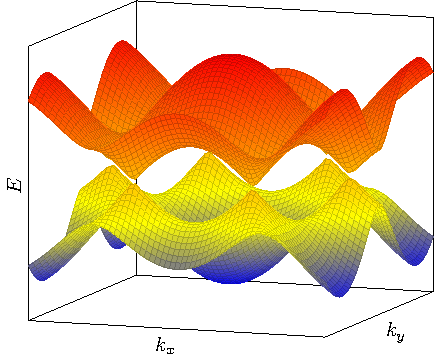
\includegraphics[width=\linewidth]{figures/bandGraphene2.pdf}
    \caption{Bandas de energía del grafeno}
    \label{fig:grapheneEnergy1}
    \end{subfigure}
    \hfill
    \begin{subfigure}[b]{0.43\linewidth}
        \centering
        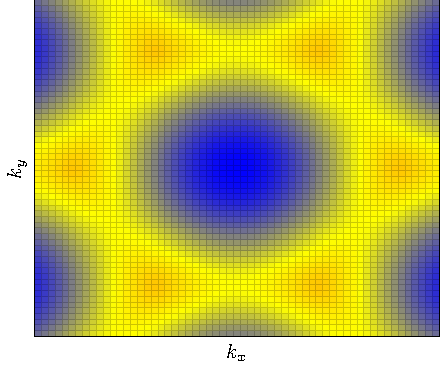
\includegraphics[width=\linewidth]{figures/bandGraphene1.pdf}
    \caption{Puntos de Dirac}
    \label{fig:grapheneEnergy2}
    \end{subfigure}
    \caption{Bandas de energía del grafeno y espectro de energía alrededor de los primeros puntos de Dirac}
\end{figure}
% ──────────────────────────────────────────────────────────────────────
\\Para hallar los valores de los puntos de Dirac se expresa $E(\vec{k})$ en función de $\vec{a}_1$ y $\vec{a}_2$.
\begin{align}
	\nonumber E(\vec{k}) & = \pm \hbar t \sqrt{3+2 \cos\left(\frac{a \sqrt{3}k_x}{2}+\frac{3ak_y}{2}\right)+2 \cos\left(-\frac{a \sqrt{3}k_x}{2}+\frac{3ak_y}{2}\right)+2 \cos\left(a \sqrt{3}k_x\right)} \\
	\nonumber            & = \pm \hbar t \sqrt{3+4 \cos\left(\frac{3ak_y}{2}\right) \cos\left(\frac{a\sqrt{3}k_x}{2}\right)+2\left[2 \cos^{2}\left(\frac{a \sqrt{3}k_x}{2}\right)-1\right]}               \\
	                     & = \pm \hbar t \sqrt{1+4 \cos\left(\frac{3ak_y}{2}\right) \cos\left(\frac{a\sqrt{3}k_x}{2}\right)+4 \cos^{2}\left(\frac{a \sqrt{3}k_x}{2}\right)}
\end{align}
Al completar cuadrados se nota que $E(\vec{k})$ es cero cuando
\begin{equation}
	\left(2 \cos\left(\frac{a\sqrt{3}k_x}{2}\right)+\cos\left(\frac{3ak_y}{2}\right)\right)^2+ \sin^2\left(\frac{3ak_y}{2}\right) = 0
\end{equation}
Entonces
\begin{equation}
	k_y = \frac{2n \pi}{3a}\quad \text{y}\quad\cos\left(\frac{a\sqrt{3}k_x}{2}\right)=\frac{\left(-1\right)^{n+1}}{2}
\end{equation}
donde $n \in \mathbb{Z}$.\\
Si $n$ es par se tiene que $k_x = \frac{4m\pi}{a\sqrt{3}}\pm \frac{4\pi}{3\sqrt{3}a}$, para $m \in \mathbb{Z}$. Entonces al expresarlo en función de los valores de $\vec{a}_1^{\ast}$ y $\vec{a}_2^{\ast}$ definidos en \eqref{eq:recipprimitive} se obtiene
\begin{equation}
	\vec{k} = \left(\frac{4m\pi}{a\sqrt{3}}\pm \frac{4\pi}{3\sqrt{3}a}\right)\hat{x} + \frac{2n\pi}{3a}\hat{y} = \begin{cases}
		(\vec{a}_1^{\ast} - \vec{a}_2^{\ast})m + (\vec{a}_1^{\ast} + \vec{a}_2^{\ast})\frac{n}{2}-\vec{a}_2^{\ast}- \frac{2\pi}{3\sqrt{3}a}\hat{x}+\frac{2\pi}{3a}\hat{y} \\
		(\vec{a}_1^{\ast} - \vec{a}_2^{\ast})m + (\vec{a}_1^{\ast} + \vec{a}_2^{\ast})\frac{n}{2}-\vec{a}_1^{\ast}+ \frac{2\pi}{3\sqrt{3}a}\hat{x}+\frac{2\pi}{3a}\hat{y}
	\end{cases}
\end{equation}
De igual forma se obtiene para $n$ impar que $k_x = \frac{4m\pi}{a\sqrt{3}}\pm \frac{2\pi}{3\sqrt{3}a}$ y
\begin{equation}
	\vec{k} = \left(\frac{4m\pi}{a\sqrt{3}}\pm \frac{2\pi}{3\sqrt{3}a}\right)\hat{x} + \frac{2n\pi}{3a}\hat{y} = \begin{cases}
		(\vec{a}_1^{\ast} - \vec{a}_2^{\ast})m + (\vec{a}_1^{\ast} + \vec{a}_2^{\ast})\frac{(n-1)}{2}- \frac{2\pi}{3\sqrt{3}a}\hat{x}+\frac{2\pi}{3a}\hat{y} \\
		(\vec{a}_1^{\ast} - \vec{a}_2^{\ast})m + (\vec{a}_1^{\ast} + \vec{a}_2^{\ast})\frac{(n-1)}{2}+ \frac{2\pi}{3\sqrt{3}a}\hat{x}+\frac{2\pi}{3a}\hat{y}
	\end{cases}
\end{equation}
Se puede observar que las soluciones son los vértices de la red recíproca del grafeno, ya que estos se pueden expresar como
\begin{equation}
	\vec{k} = m' \vec{a}_1^{\ast}+ n' \vec{a}_2^{\ast} \pm \frac{2\pi}{3\sqrt{3}}\hat{x}+\frac{2\pi}{3a}\hat{y}
\end{equation}
donde $m$ y $n$ son números enteros.\par
Así se definen los conjuntos de puntos de Dirac dados por
\begin{equation}
	[\vec{K}^{+}] = \left\{\vec{K}^{+}_{mn}\mid \vec{K}^{+}_{mn} =m \vec{a}_1^{\ast}+ n \vec{a}_2^{\ast} + \frac{2\pi}{3\sqrt{3}}\hat{x}+\frac{2\pi}{3a}\hat{y},\text{ donde }m,n \in \mathbb{Z} \right\}\label{eq:diracpointequiv1}
\end{equation}
\begin{equation}
	[\vec{K}^{-}] = \left\{\vec{K}^{-}_{mn}\mid \vec{K}^{-}_{mn} =m \vec{a}_1^{\ast}+ n \vec{a}_2^{\ast} - \frac{2\pi}{3\sqrt{3}}\hat{x}+\frac{2\pi}{3a}\hat{y},\text{ donde }m,n \in \mathbb{Z} \right\}\label{eq:diracpointequiv2}
\end{equation}
Estos forman las dos sub-redes triangulares de la red recíproca.
\subsection{Espectro de energía alrededor de los puntos de Dirac}
Para hallar de manera aproximada el valor de la energía alrededor de los puntos de Dirac se define $\vec{\kappa} = \vec{k}-\vec{K}^{\pm}_{mn}$, tal que $\left\lVert \vec{\kappa}\right\rVert\ll 1$, y se realiza la expansión de Taylor de $f(\vec{k})$ alrededor del punto $\vec{K}^{\pm}_{mn}$.
\begin{align}
	\nonumber	f(\vec{k}) & = 1+e^{-i\vec{K}^{\pm}_{mn}\cdot \vec{a}_1}e^{-i \vec{\kappa}\cdot \vec{a}_1}+e^{-i \vec{K}^{\pm}_{mn}\cdot \vec{a}_2}e^{-i \vec{\kappa}\cdot \vec{a}_2}                                                                                                                                                                                                               \\
	\nonumber            & =1+e^{-i\vec{K}^{\pm}_{mn}\cdot \vec{a}_1}\resizebox{0.3\textwidth}{!}{$\left(1-i \vec{\kappa}\cdot \vec{a}_1 - \frac{\left(\vec{\kappa}\cdot \vec{a}_1\right)^2}{2}+\ldots\right)$}+e^{-i\vec{K}^{\pm}_{mn}\cdot \vec{a}_2}\resizebox{0.3\textwidth}{!}{$\left(1-i \vec{\kappa}\cdot \vec{a}_2 - \frac{\left(\vec{\kappa}\cdot \vec{a}_2\right)^2}{2}+\ldots\right)$} \\
	                     & \approx 1+e^{-i \vec{K}^{\pm}_{mn}\cdot \vec{a}_1}+e^{-i \vec{K}^{\pm}_{mn}\cdot \vec{a}_2}-i \vec{\kappa}\cdot \vec{a}_1e^{-i \vec{K}^{\pm}_{mn}\cdot \vec{a}_1}-i \vec{\kappa}\cdot \vec{a}_2 e^{-i \vec{K}^{\pm}_{mn}\cdot \vec{a}_2}
\end{align}
Ya que la energía en los puntos de Dirac es cero, es decir $\abs{f(\vec{K}^{\pm}_{mn}})=0$, se obtiene
\begin{equation}
	f(\vec{k}) \approx -i (\vec{\kappa}\cdot \vec{a}_1) e^{-i \vec{K}^{\pm}_{mn}\cdot \vec{a}_1} -i( \vec{\kappa}\cdot \vec{a}_2) e^{-i \vec{K}^{\pm}_{mn} \cdot \vec{a}_2}
\end{equation}
Para $\vec{K}^{+}_{mn}$
\begin{align}
	\nonumber f(\vec{k}) & = -i \left(\frac{a\sqrt{3}}{2}\kappa_1+\frac{3a}{2}\kappa_2\right)e^{-i 4\pi/3-i2\pi m}-i \left(-\frac{a\sqrt{3}}{2}\kappa_1 + \frac{3a}{2}\kappa_2\right)e^{-i 2\pi/3-i2\pi n}                                                     \\
	\nonumber            & = -i \left(\frac{a\sqrt{3}}{2}\kappa_1+\frac{3a}{2}\kappa_2\right)\left(-\frac{1}{2}+i \frac{\sqrt{3}}{2} \right)-i \left(-\frac{a\sqrt{3}}{2}\kappa_1 + \frac{3a}{2}\kappa_2\right)\left(-\frac{1}{2}-i \frac{\sqrt{3}}{2} \right) \\
                       & = \frac{3a}{2}\left(\kappa_1+i\kappa_2\right)\label{eq:firstApproxEnergy1}
\end{align}
Para $\vec{K}^{-}_{mn}$
\begin{align}
	\nonumber f(\vec{k}) & = -i \left(\frac{a\sqrt{3}}{2}\kappa_1+\frac{3a}{2}\kappa_2\right)e^{-i 2\pi/3-i2\pi m}-i \left(-\frac{a\sqrt{3}}{2}\kappa_1 + \frac{3a}{2}\kappa_2\right)e^{-i 4\pi/3-i2\pi n}                                                     \\
	\nonumber            & = -i \left(\frac{a\sqrt{3}}{2}\kappa_1+\frac{3a}{2}\kappa_2\right)\left(-\frac{1}{2}-i \frac{\sqrt{3}}{2} \right)-i \left(-\frac{a\sqrt{3}}{2}\kappa_1 + \frac{3a}{2}\kappa_2\right)\left(-\frac{1}{2}+i \frac{\sqrt{3}}{2} \right) \\
                       & =  \frac{3a}{2}\left(-\kappa_1+i\kappa_2\right)\label{EQ:firstApproxEnergy2}
\end{align}
Reemplazando en \eqref{eq:energygraphene} se obtiene 
\begin{equation}
   E(\vec{k}) = \pm \frac{3\hbar a t}{2} \sqrt{\kappa_1^2 + \kappa_2^2},
\end{equation}
por lo que los valores de la energía alrededor de los puntos de Dirac es independiente del conjunto de puntos Dirac que se elija. Además la forma del espectro energía alrededor de los puntos de Dirac toma la forma de un cono, lo cual es consistente con el hecho de que sean llamados como \emph{conos de Dirac}.
